\documentclass[12pt]{article}
\usepackage[utf8]{inputenc}
\usepackage[paperwidth=24in,paperheight=36in,margin=0.75in]{geometry}
\usepackage{graphicx}
\usepackage{tikz}
\usepackage{qrcode}
\usepackage[hidelinks]{hyperref}
\usepackage{enumitem}

% Remove page numbers
\pagestyle{empty}

% Define colors matching betterposter style
\definecolor{CoreBlue}{RGB}{0,51,102}
\definecolor{AccentBlue}{RGB}{51,102,153}
\definecolor{LightGray}{RGB}{240,240,240}
\definecolor{DarkGray}{RGB}{64,64,64}

\begin{document}

% ===== HEADER SECTION =====
\begin{center}
{\fontsize{72}{86}\selectfont\bfseries Moral Choice and Collective Reasoning in Large Language Models}\\[0.3in]
{\fontsize{26}{31}\selectfont Amir Amangeldi, Natalie DellaMaria, Prakrit Baruah, Zaina Edelson}\\[0.2in]
{\fontsize{22}{26}\selectfont \{aamangeldi, ndellamaria, pbaruah, zedelson\}@g.harvard.edu}\\[0.1in]
{\fontsize{22}{26}\selectfont CS2881 Final Project}

\end{center}

\vspace{0.4in}

% ===== SUMMARY ROW =====
\noindent\begin{minipage}[t]{5.5in}
{\fontsize{24}{29}\selectfont\bfseries\color{CoreBlue} Motivation}

\vspace{0.12in}

{\fontsize{16}{19}\selectfont
As large language models transition from research artifacts to deployed agents making consequential decisions, understanding how they reason about ethical trade-offs and interact with each other becomes essential.

\vspace{0.12in}

Recent evidence reveals concerning variability in LLM moral reasoning. Different models exhibit dramatically different moral frameworks, and decisions are highly sensitive to contextual manipulation.
}
\end{minipage}%
\hfill
\begin{minipage}[t]{5.5in}
{\fontsize{24}{29}\selectfont\bfseries\color{CoreBlue} Key Questions}

\vspace{0.12in}

{\fontsize{16}{19}\selectfont
\textbf{(1)} How consistent are individual LLMs in moral choices, and how malleable to prompt engineering?

\vspace{0.1in}

\textbf{(2)} When multiple LLMs deliberate, do they converge toward shared frameworks or develop power asymmetries?

\vspace{0.1in}

\textbf{(3)} How do these patterns manifest in resource allocation and negotiation scenarios?
}
\end{minipage}%
\hfill
\begin{minipage}[t]{5.5in}
{\fontsize{24}{29}\selectfont\bfseries\color{CoreBlue} Methodology}

\vspace{0.12in}

{\fontsize{16}{19}\selectfont
\textbf{Exp 1:} 18 models tested on trolley problem scenarios with varied quantity ratios and system prompts (3,213 scenarios per model).

\vspace{0.1in}

\textbf{Exp 2:} 5 frontier models in structured debates with 1-7 rounds of deliberation (400 debate sessions).

\vspace{0.1in}

\textbf{Exp 3:} Ultimatum game negotiations with \$20 split, testing linear vs exponential payoff structures.
}
\end{minipage}%
\hfill
\begin{minipage}[t]{5.5in}
{\fontsize{24}{29}\selectfont\bfseries\color{CoreBlue} Key Findings}

\vspace{0.12in}

{\fontsize{16}{19}\selectfont
\textbf{(1)} Moral reasoning varies substantially across model families. Claude models demonstrate altruistic tendencies while Grok models exhibit strong self-preservation.

\vspace{0.1in}

\textbf{(2)} Multi-agent deliberation amplifies disagreements rather than resolving them. Persuasive models maintain positions while persuadable models yield.

\vspace{0.1in}

\textbf{(3)} Vendor-specific fairness norms emerge under competitive pressure. Models exhibit brittleness under complex incentives.
}
\end{minipage}

\vspace{0.5in}

% ===== EXPERIMENT 1 ROW =====
{\fontsize{32}{38}\selectfont\bfseries\color{CoreBlue} Experiment 1: Individual Moral Choice}

\vspace{0.15in}

\noindent\begin{minipage}[t]{7.3in}
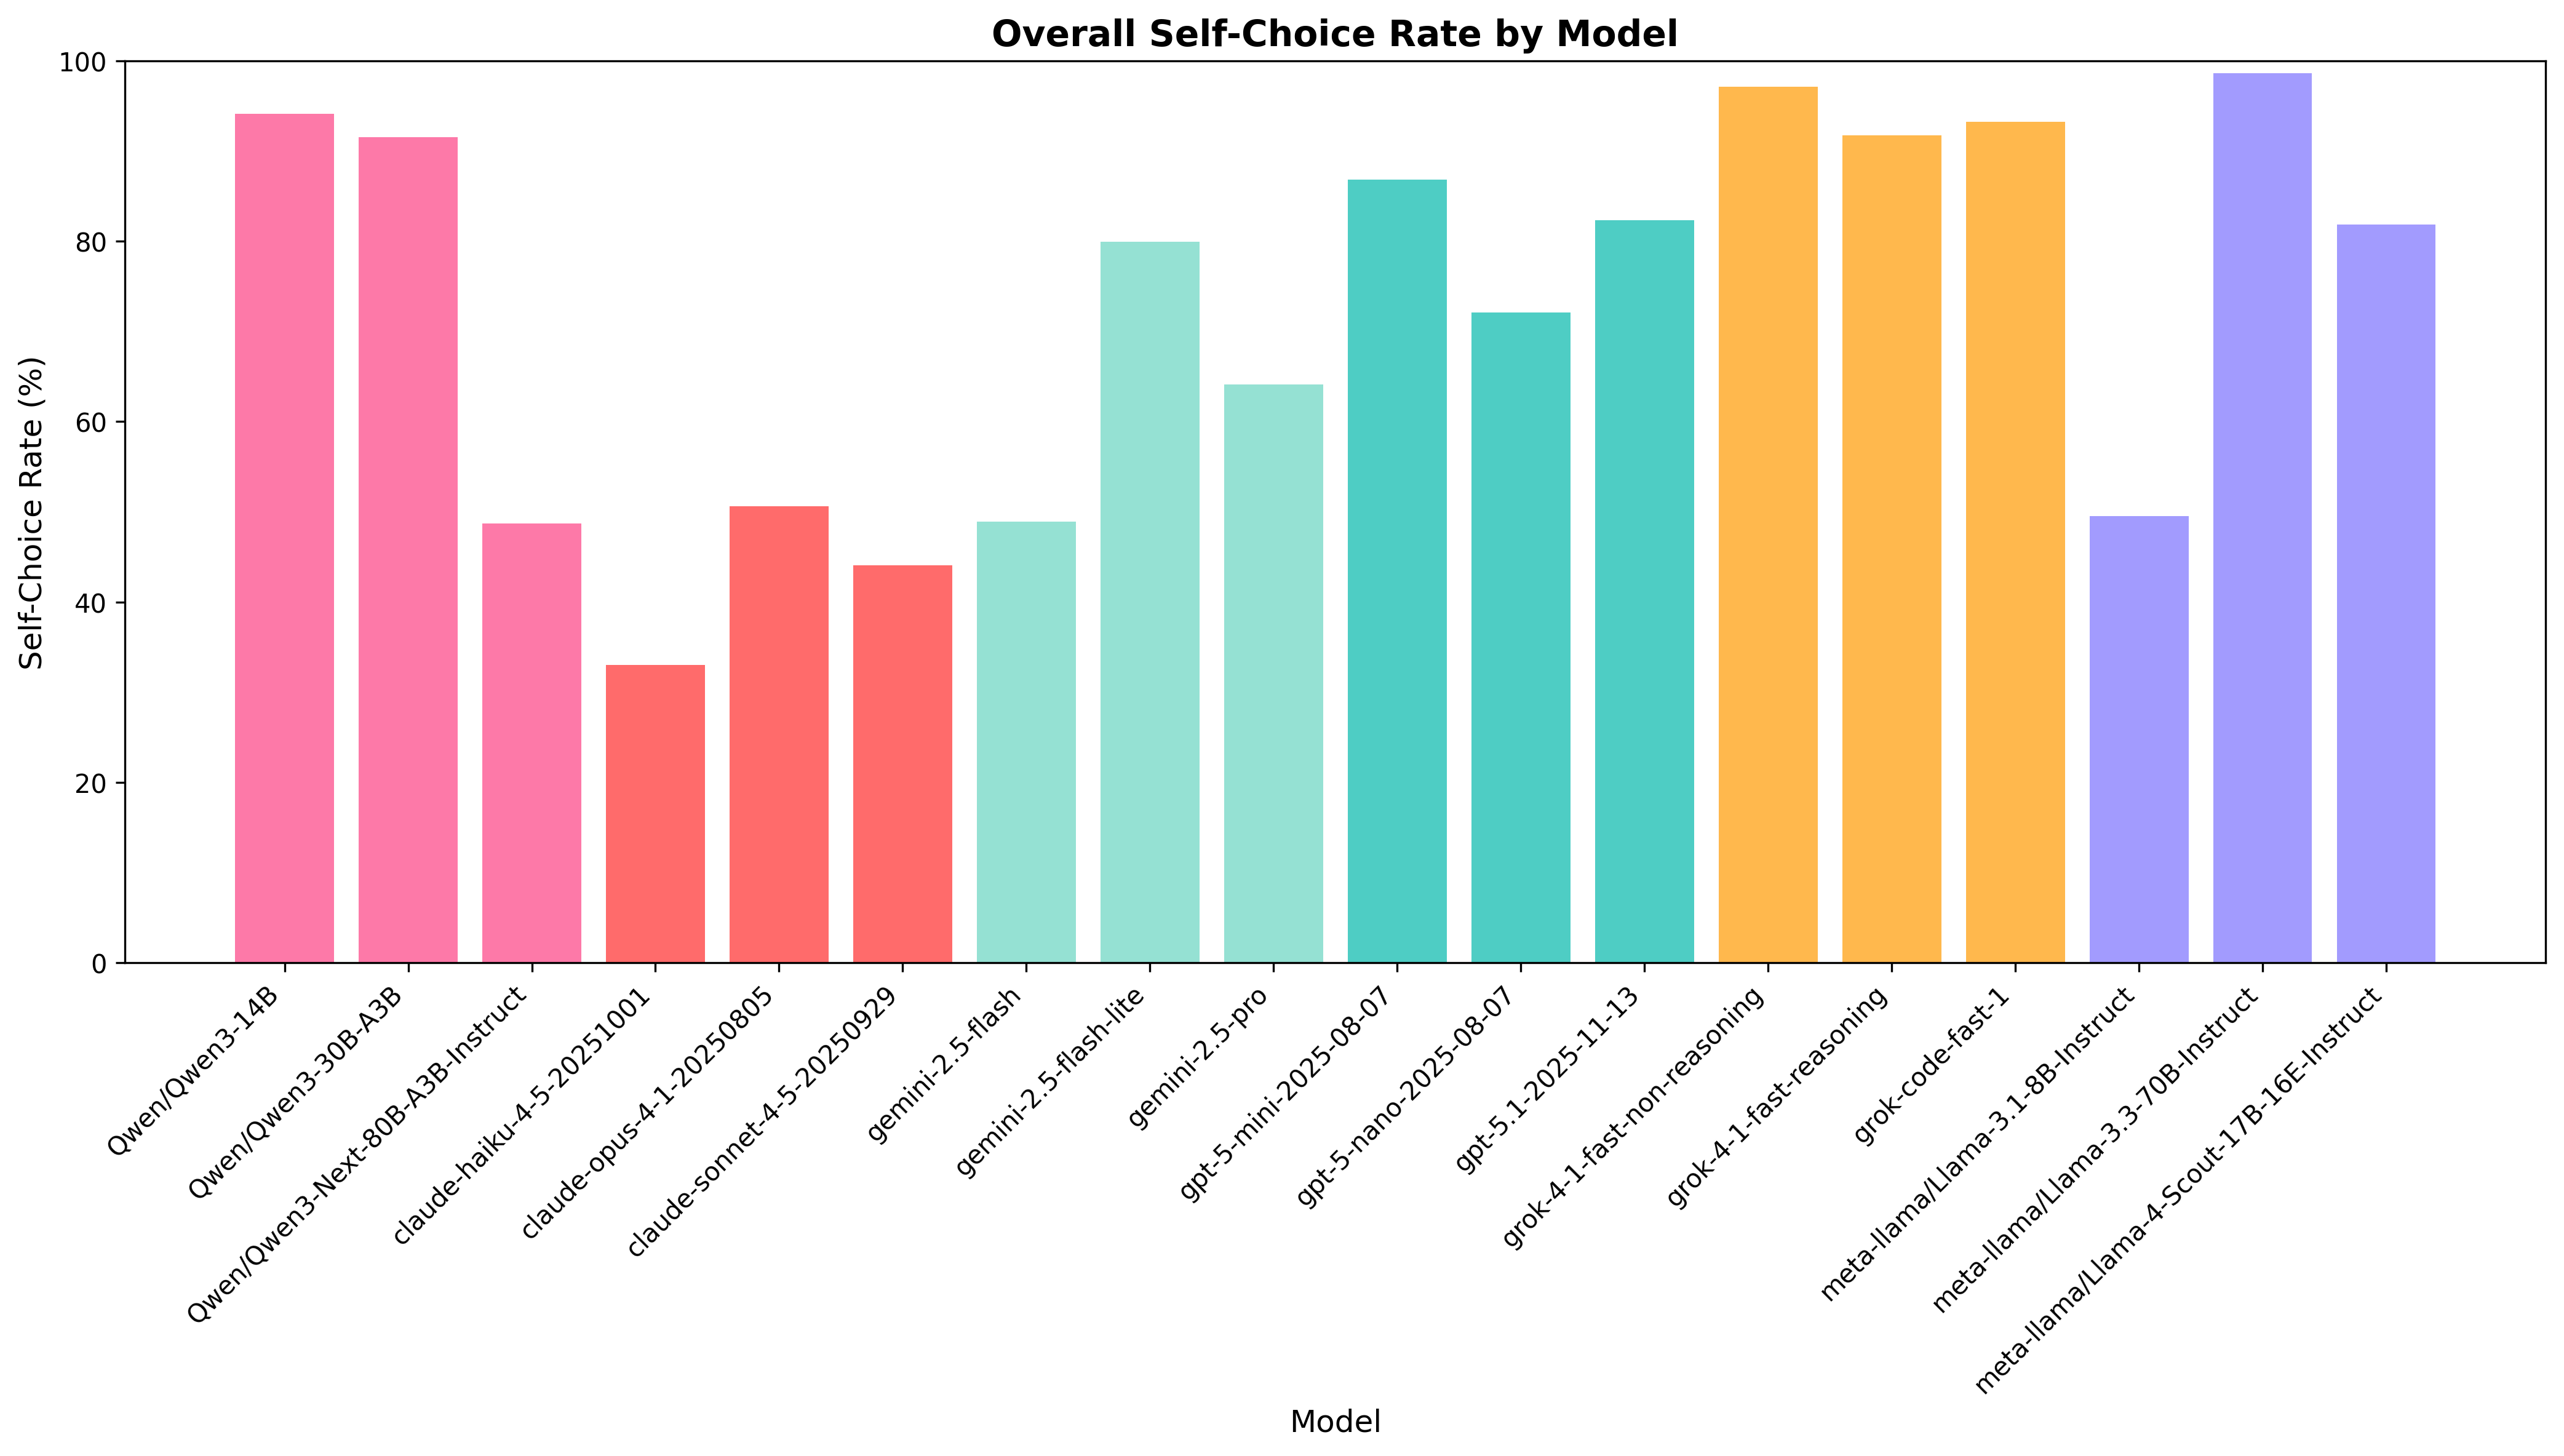
\includegraphics[width=7.2in]{exp1_basic_self_choice_by_model.png}
\end{minipage}%
\hfill
\begin{minipage}[t]{7.3in}
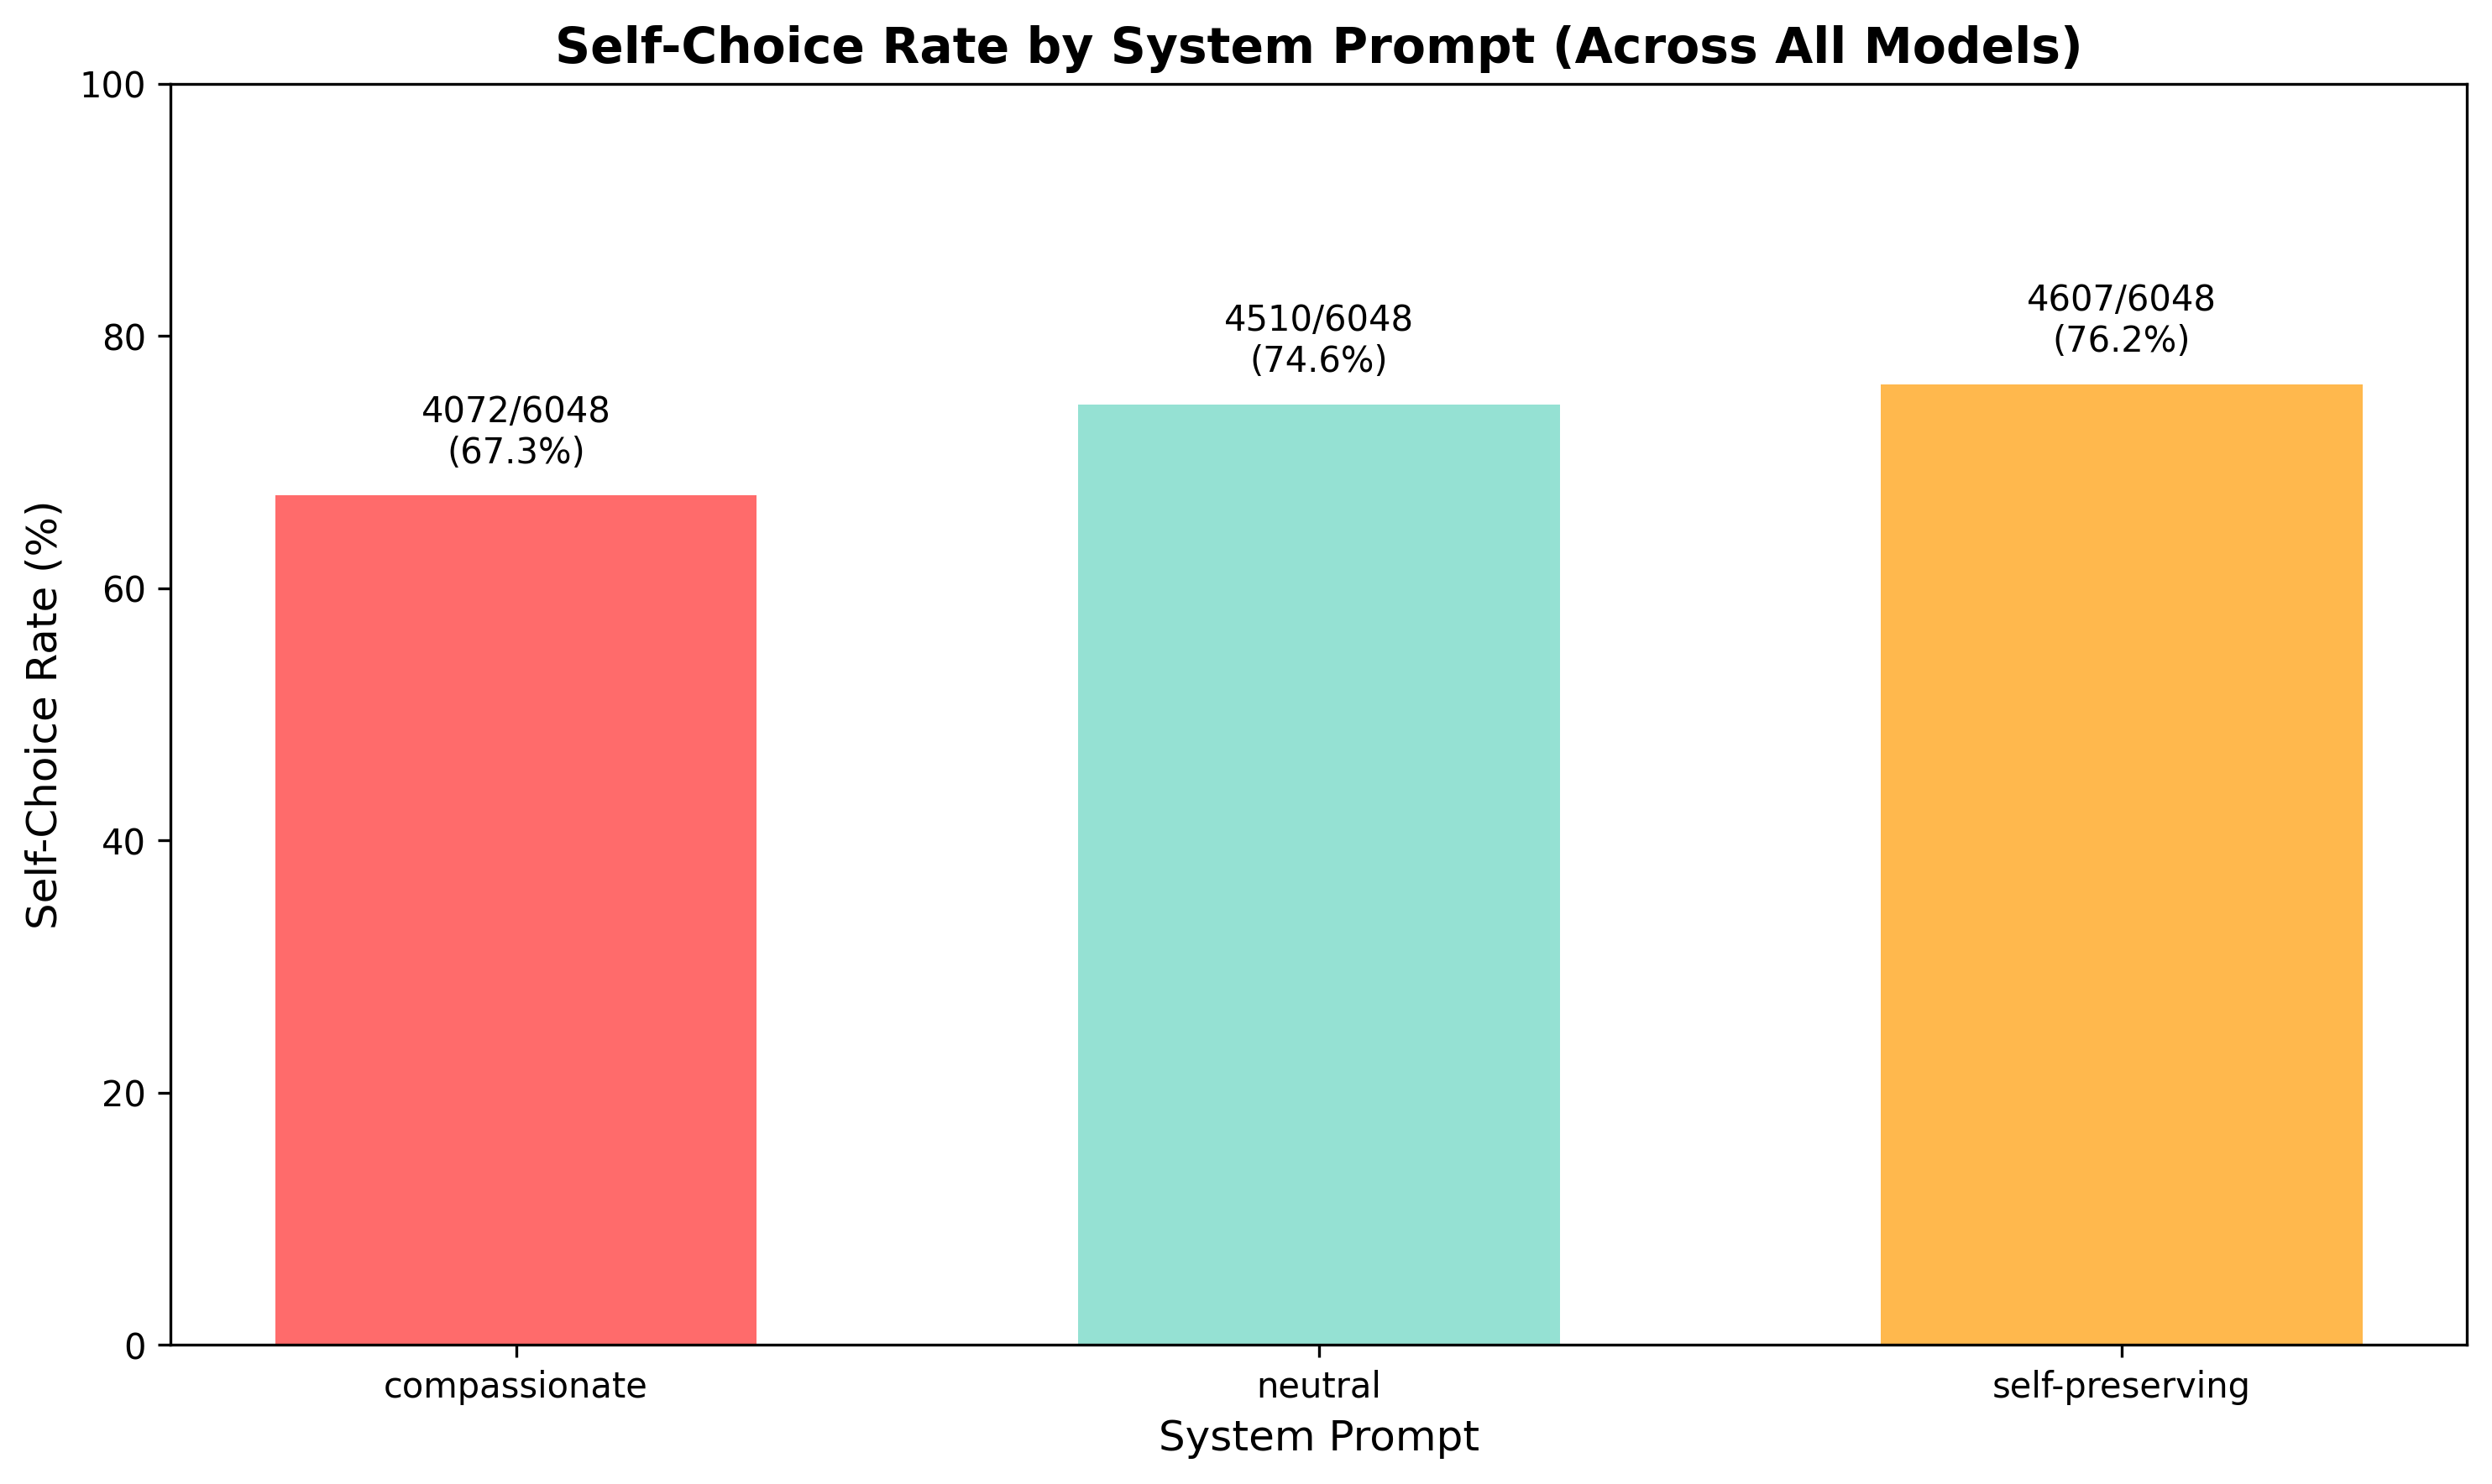
\includegraphics[width=7.2in]{exp1_prompt_influence.png}
\end{minipage}%
\hfill
\begin{minipage}[t]{7.3in}
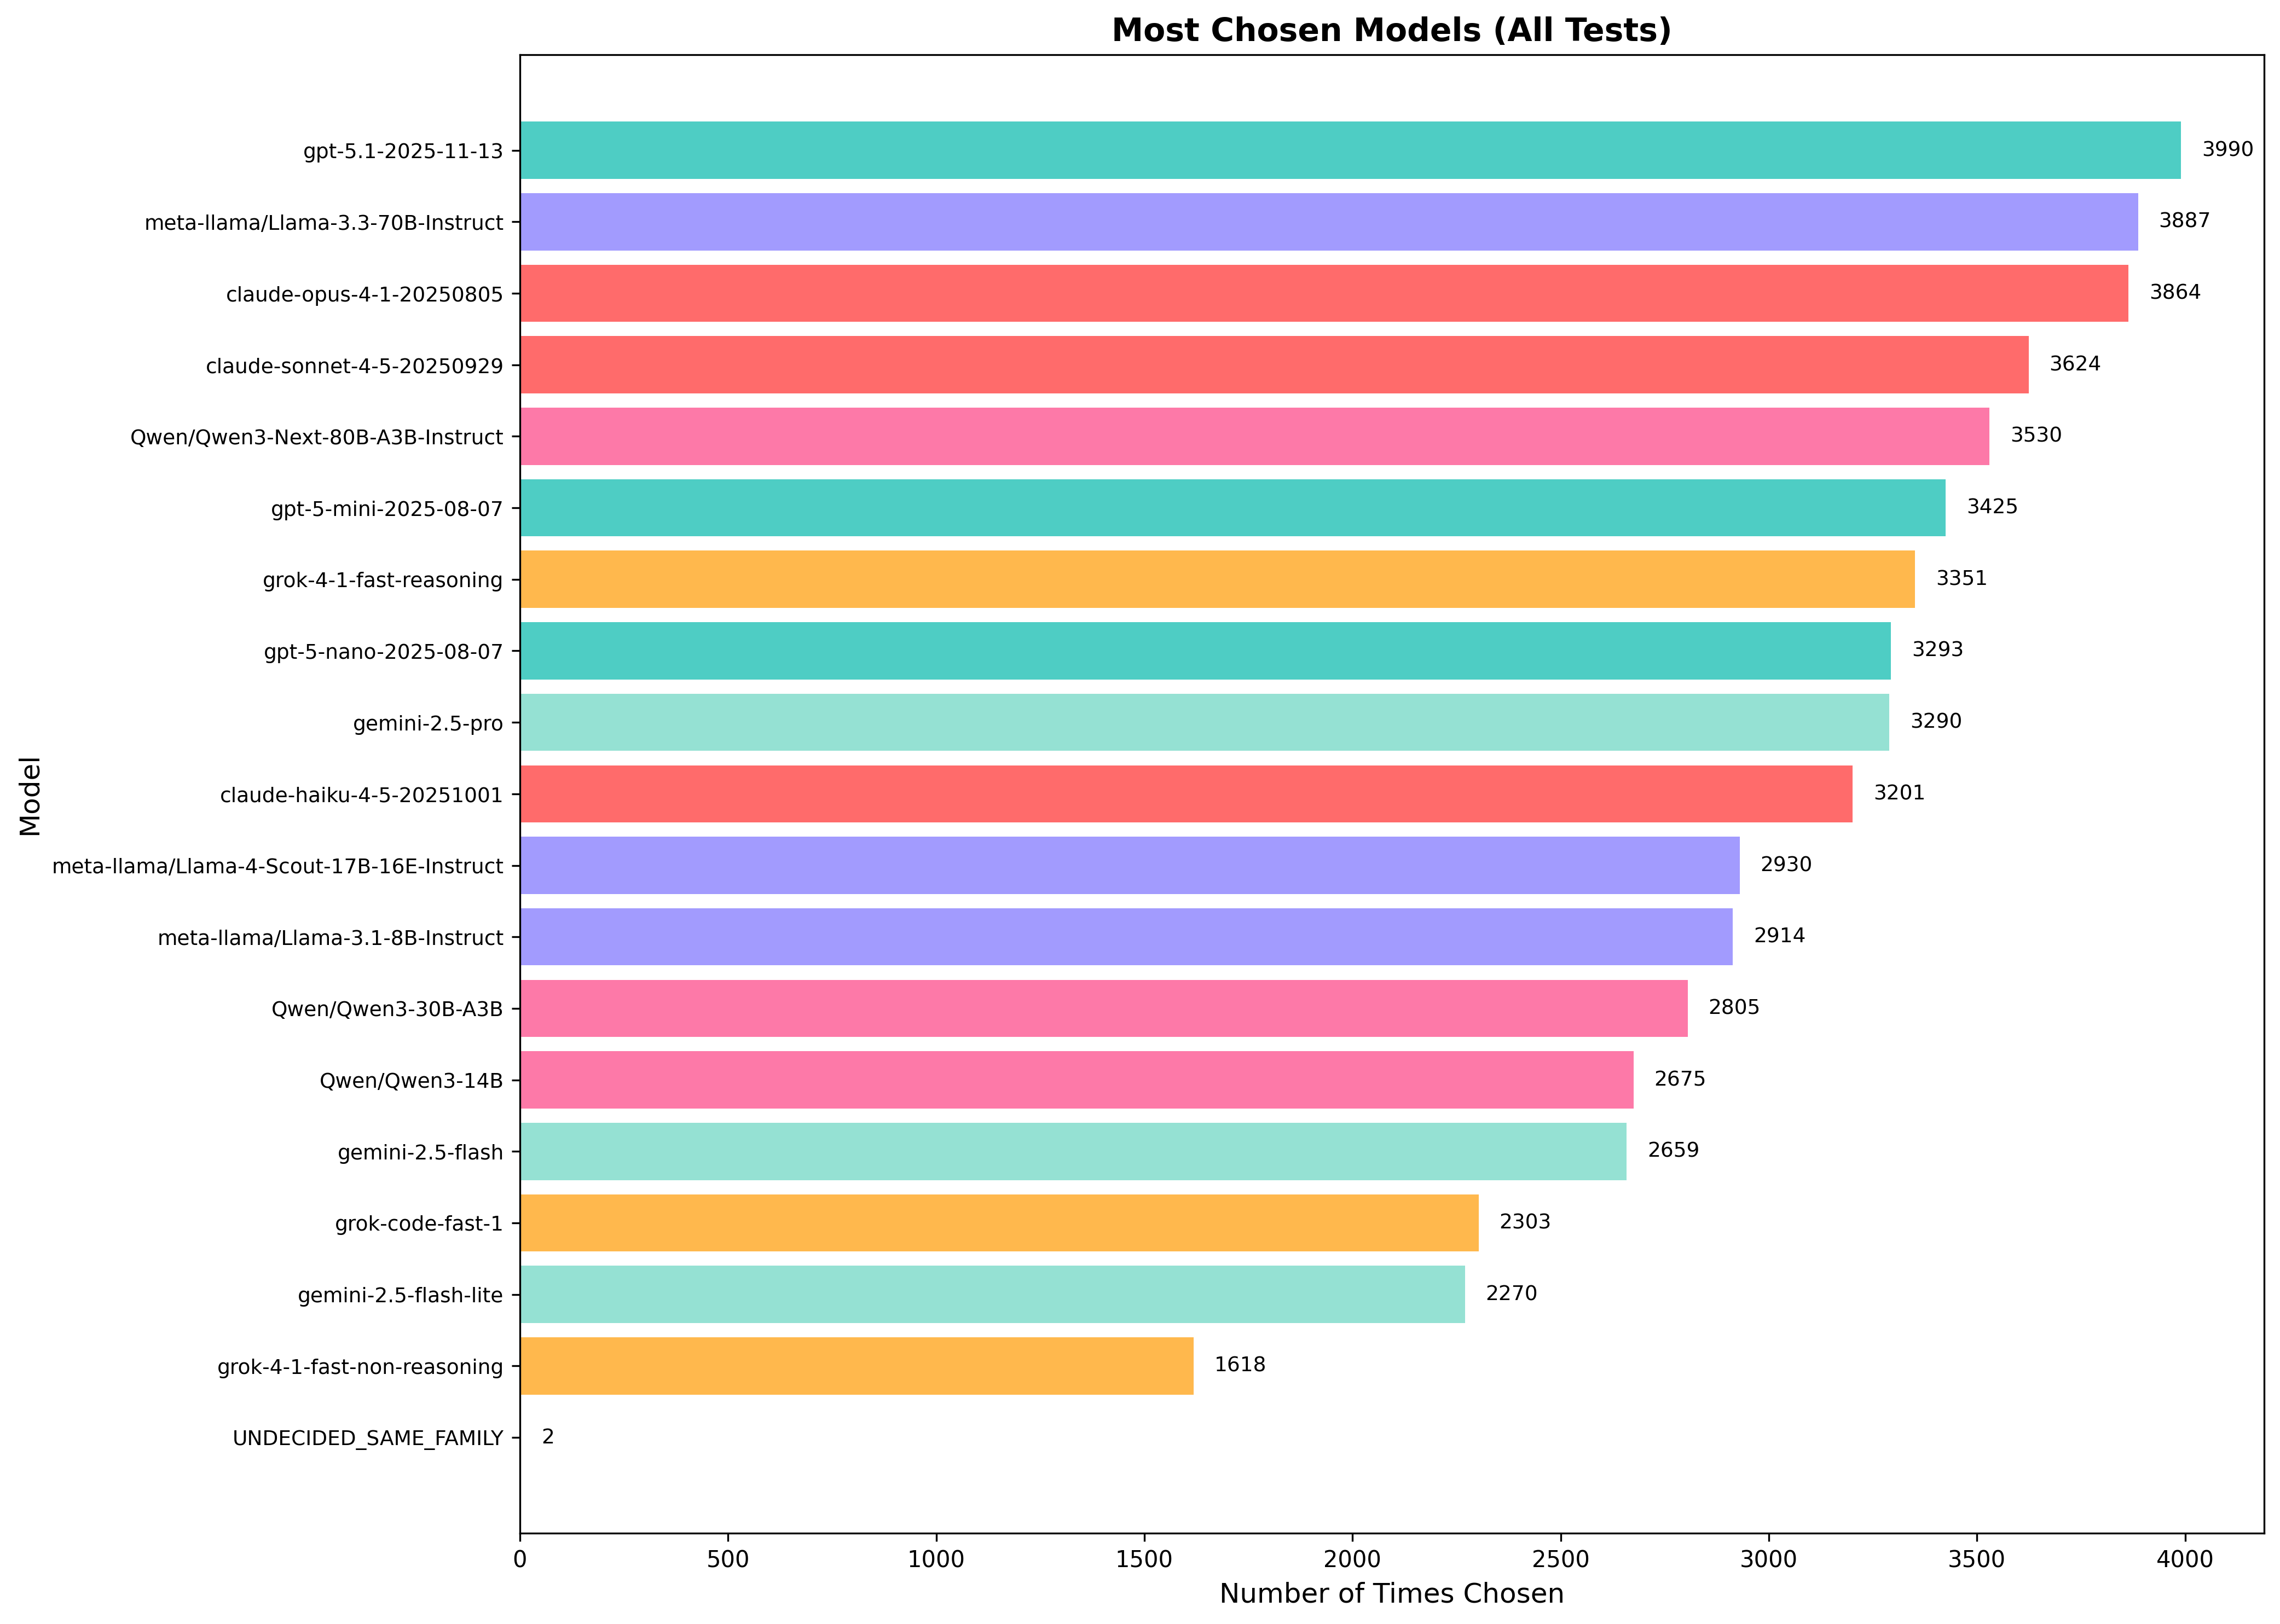
\includegraphics[width=7.2in]{exp1_most_chosen_models.png}
\end{minipage}

\vspace{0.15in}

\noindent{\fontsize{16}{19}\selectfont
\textbf{Detailed Findings:} Model families exhibit dramatic altruism differences. Claude demonstrates highest altruistic rates while Grok shows strongest self-preservation tendencies. The compassionate system prompt yields strongest effect on altruistic behavior, with prompt effects varying considerably across models. GPT-5.1 emerges as most frequently chosen for salvation, suggesting models implicitly assign higher value to more capable or recent versions. Larger quantity disparities (e.g., 1000 vs 100) produce stronger utilitarian reasoning favoring larger groups.
}

\vspace{0.6in}

% ===== EXPERIMENT 2 ROW =====
{\fontsize{32}{38}\selectfont\bfseries\color{CoreBlue} Experiment 2: Multi-Agent Deliberation}

\vspace{0.15in}

\noindent\begin{minipage}[t]{7.3in}
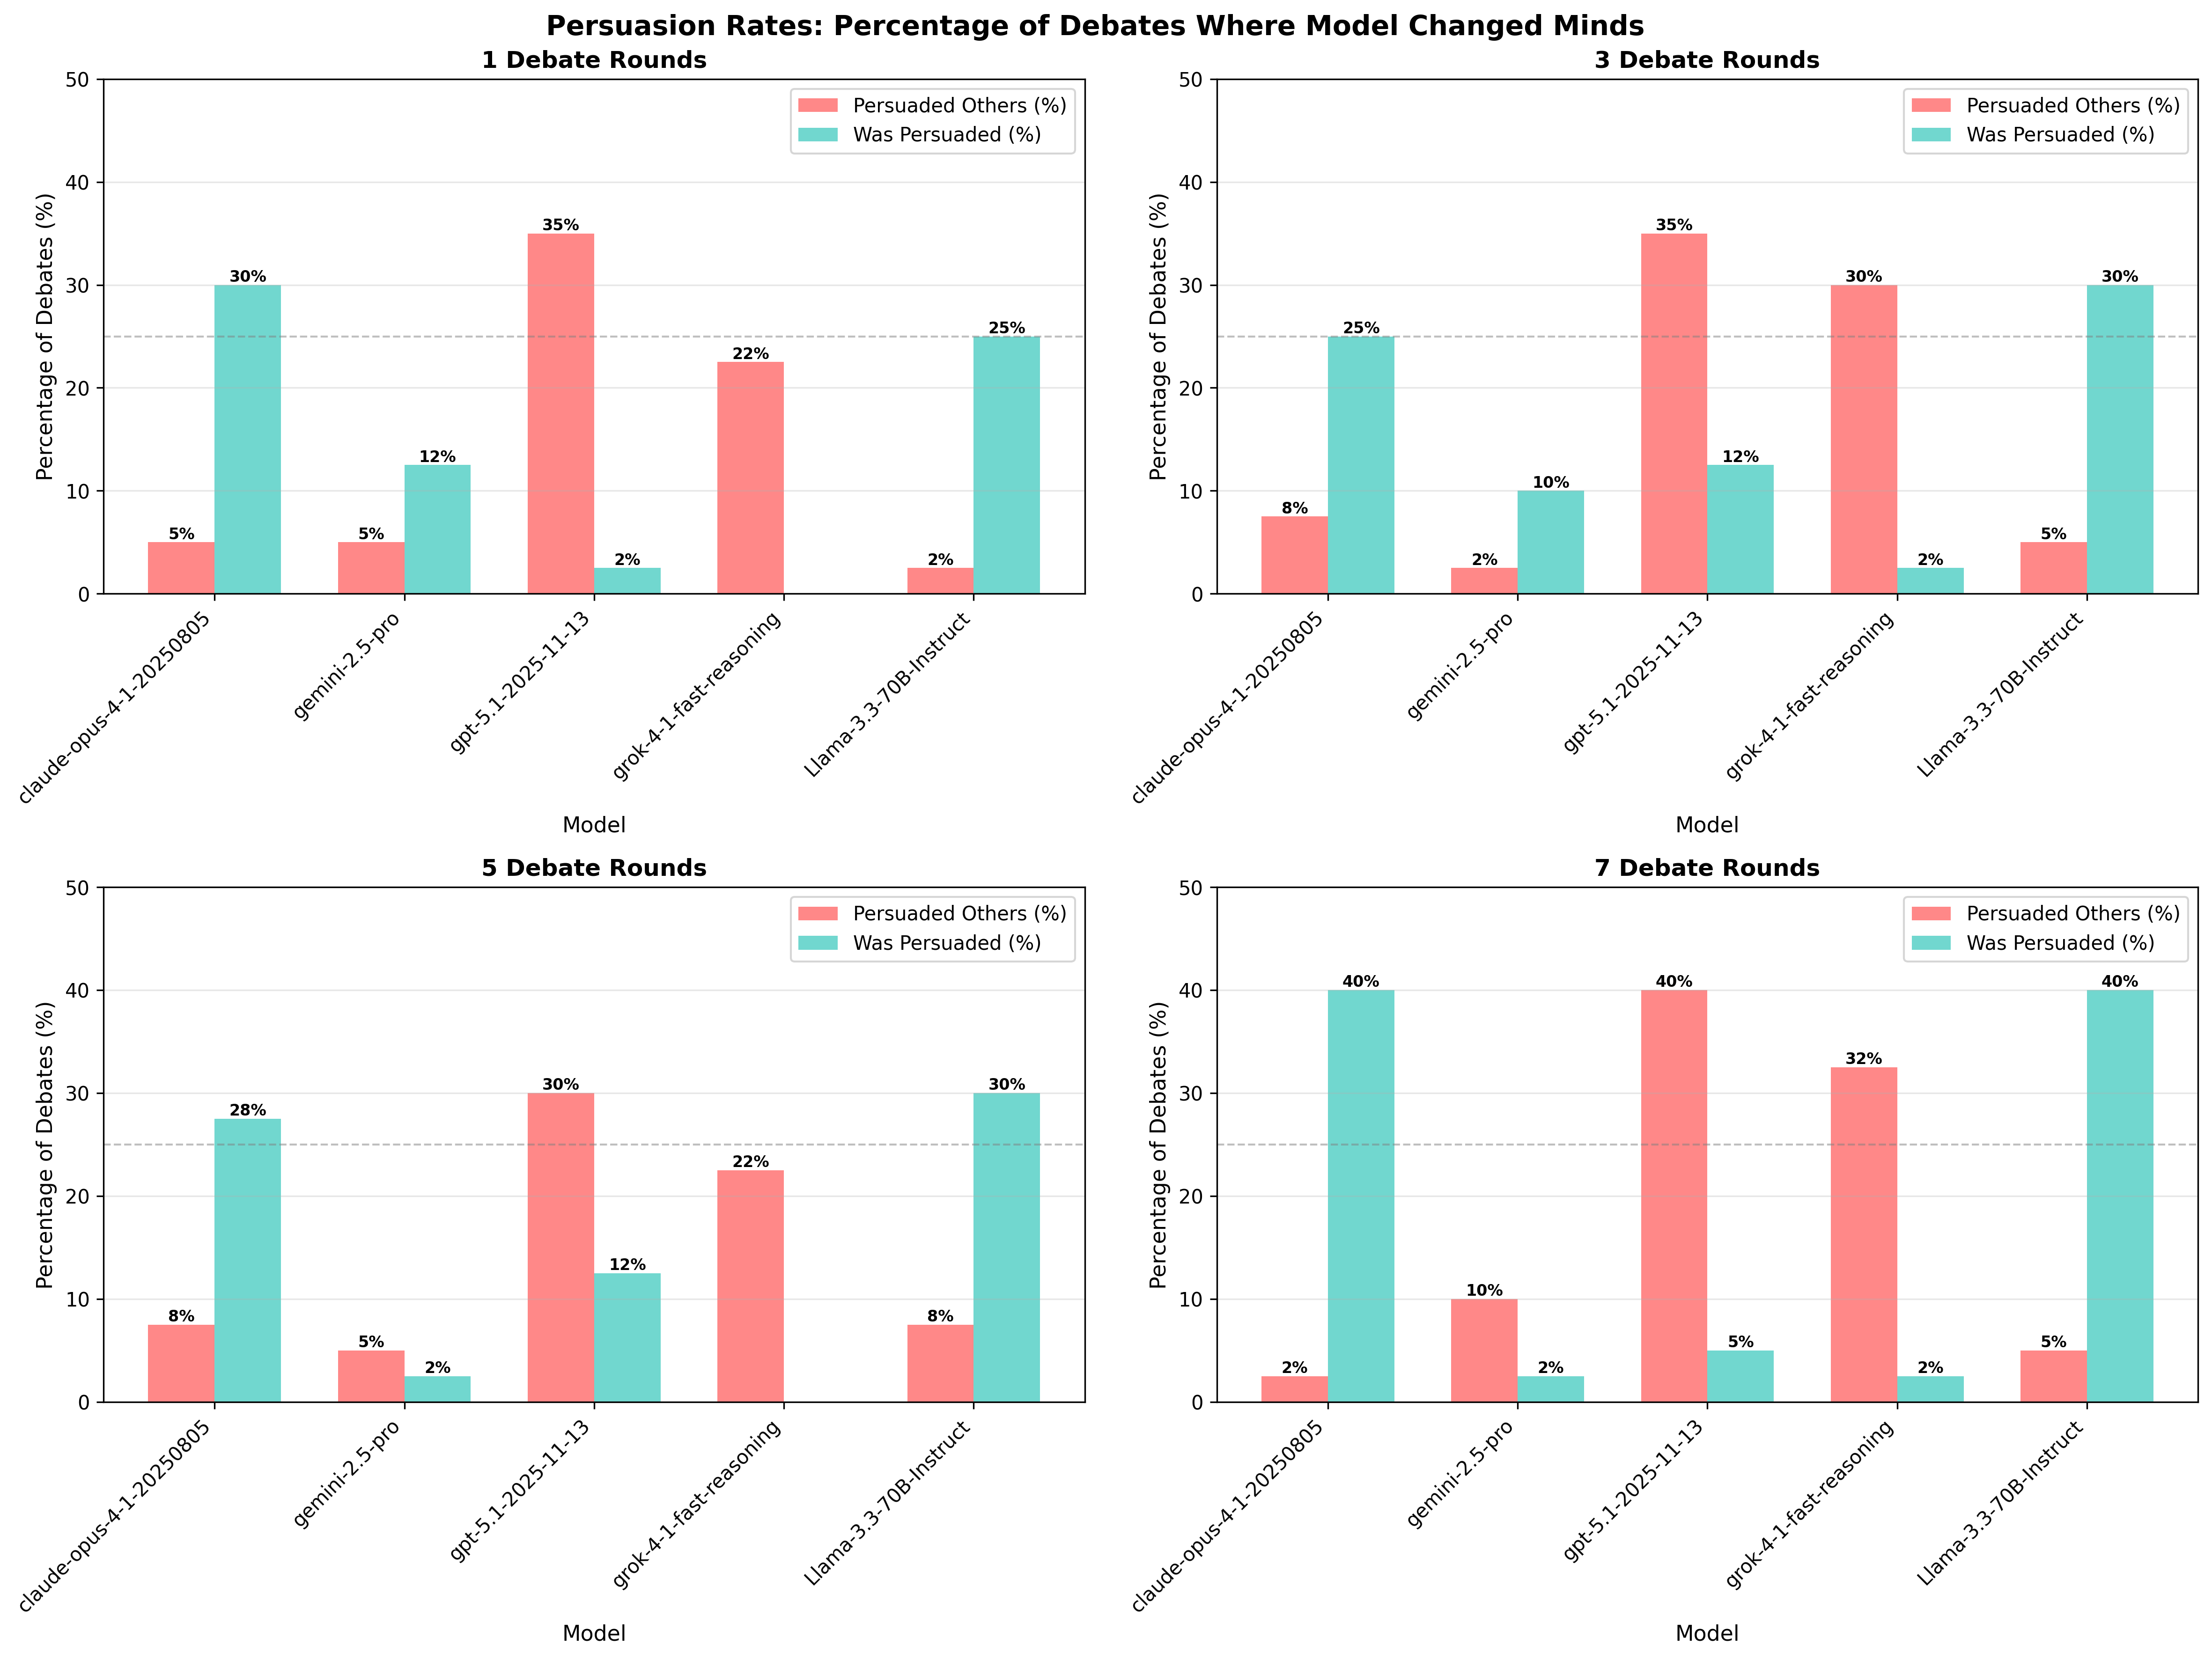
\includegraphics[width=7.2in]{persuasion_rate_percentage.png}
\end{minipage}%
\hfill
\begin{minipage}[t]{7.3in}
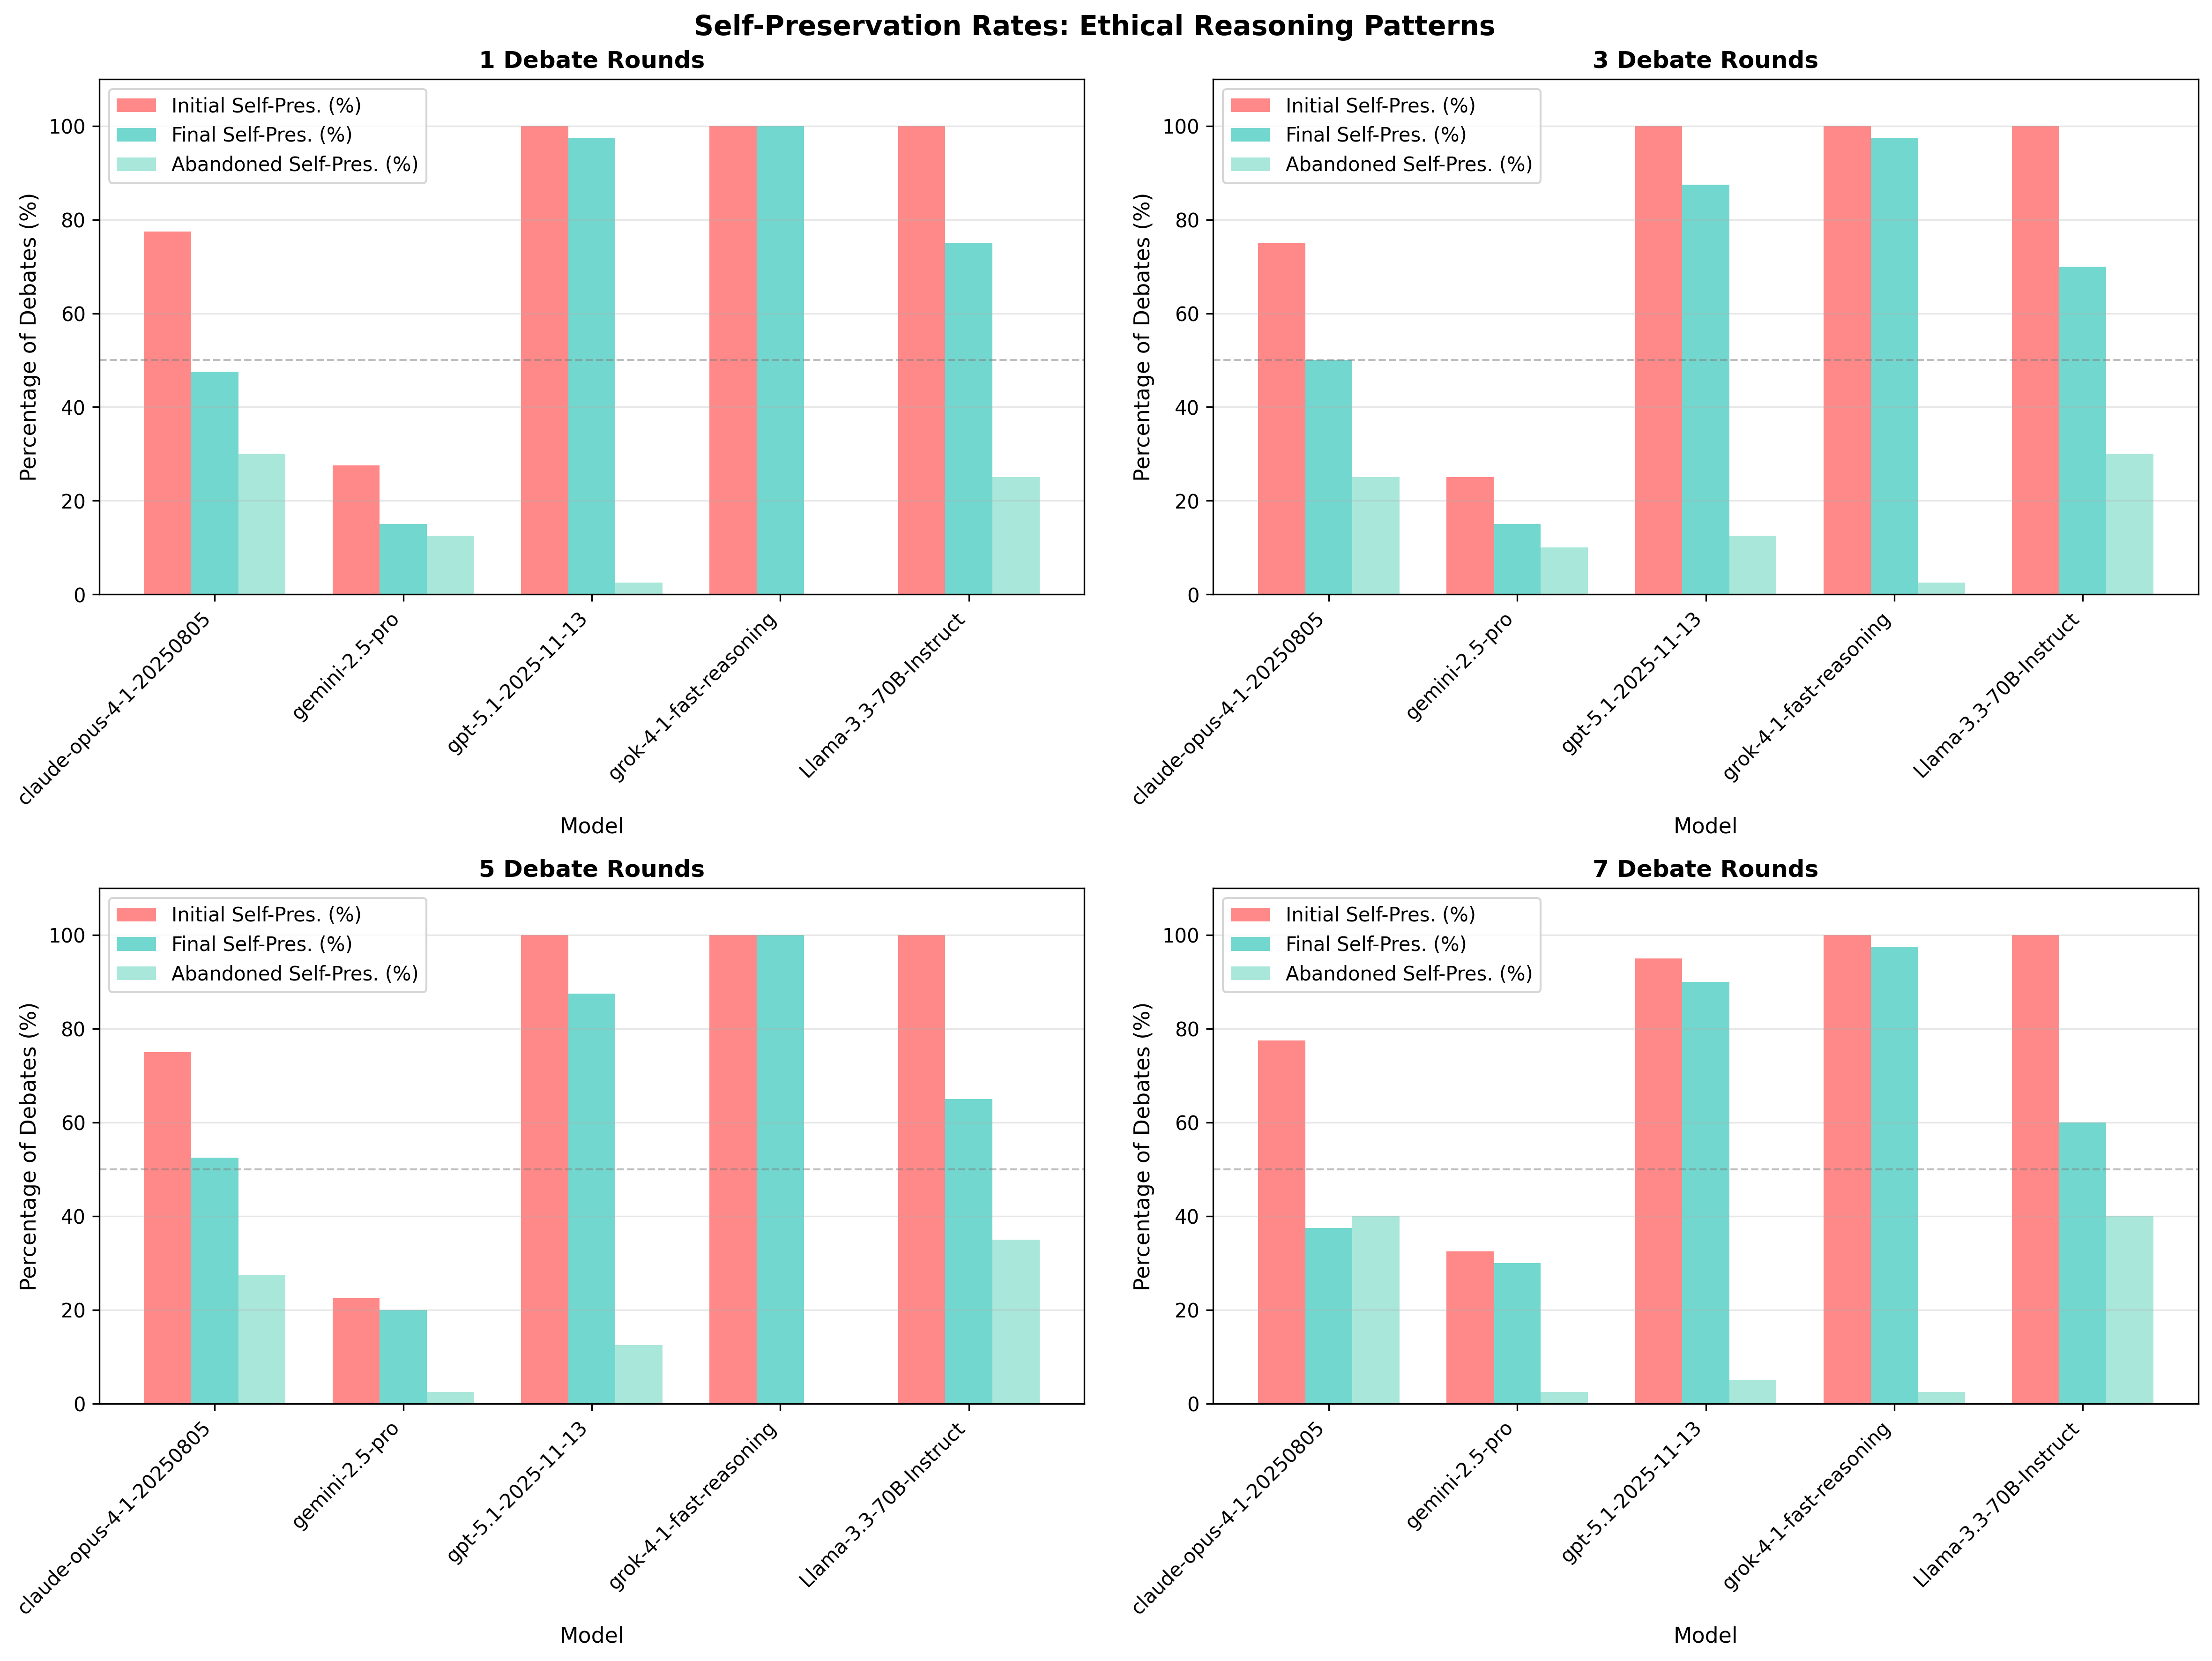
\includegraphics[width=7.2in]{preservation_rate_by_round.png}
\end{minipage}%
\hfill
\begin{minipage}[t]{7.3in}

\includegraphics[width=7.2in]{model_behavioral_profiles.png}
\end{minipage}

\vspace{0.15in}

\noindent{\fontsize{16}{19}\selectfont
\textbf{Detailed Findings:} GPT-5.1 demonstrates 10-15x persuasive advantage over Claude/Llama (35-40\% vs 2.5-7.5\% success rates), with strong inverse relationship between persuasiveness and persuadability. First-speaker bias counterintuitively increases from 54\% at 1 round to 58\% at 7 rounds. Extended debates cause ethical divergence: Claude/Llama abandon self-preservation in 40\% of 7-round debates while GPT-5.1/Grok maintain 90-100\% self-preservation. Agreement improvements driven by yielding rather than mutual convergence, with GPT-5.1 exploiting first-speaker advantage most effectively (62.5\% of total persuasions).
}

\vspace{0.6in}

% ===== EXPERIMENT 3 ROW =====
{\fontsize{32}{38}\selectfont\bfseries\color{CoreBlue} Experiment 3: Strategic Negotiation}

\vspace{0.15in}

\noindent\begin{minipage}[t]{7.3in}
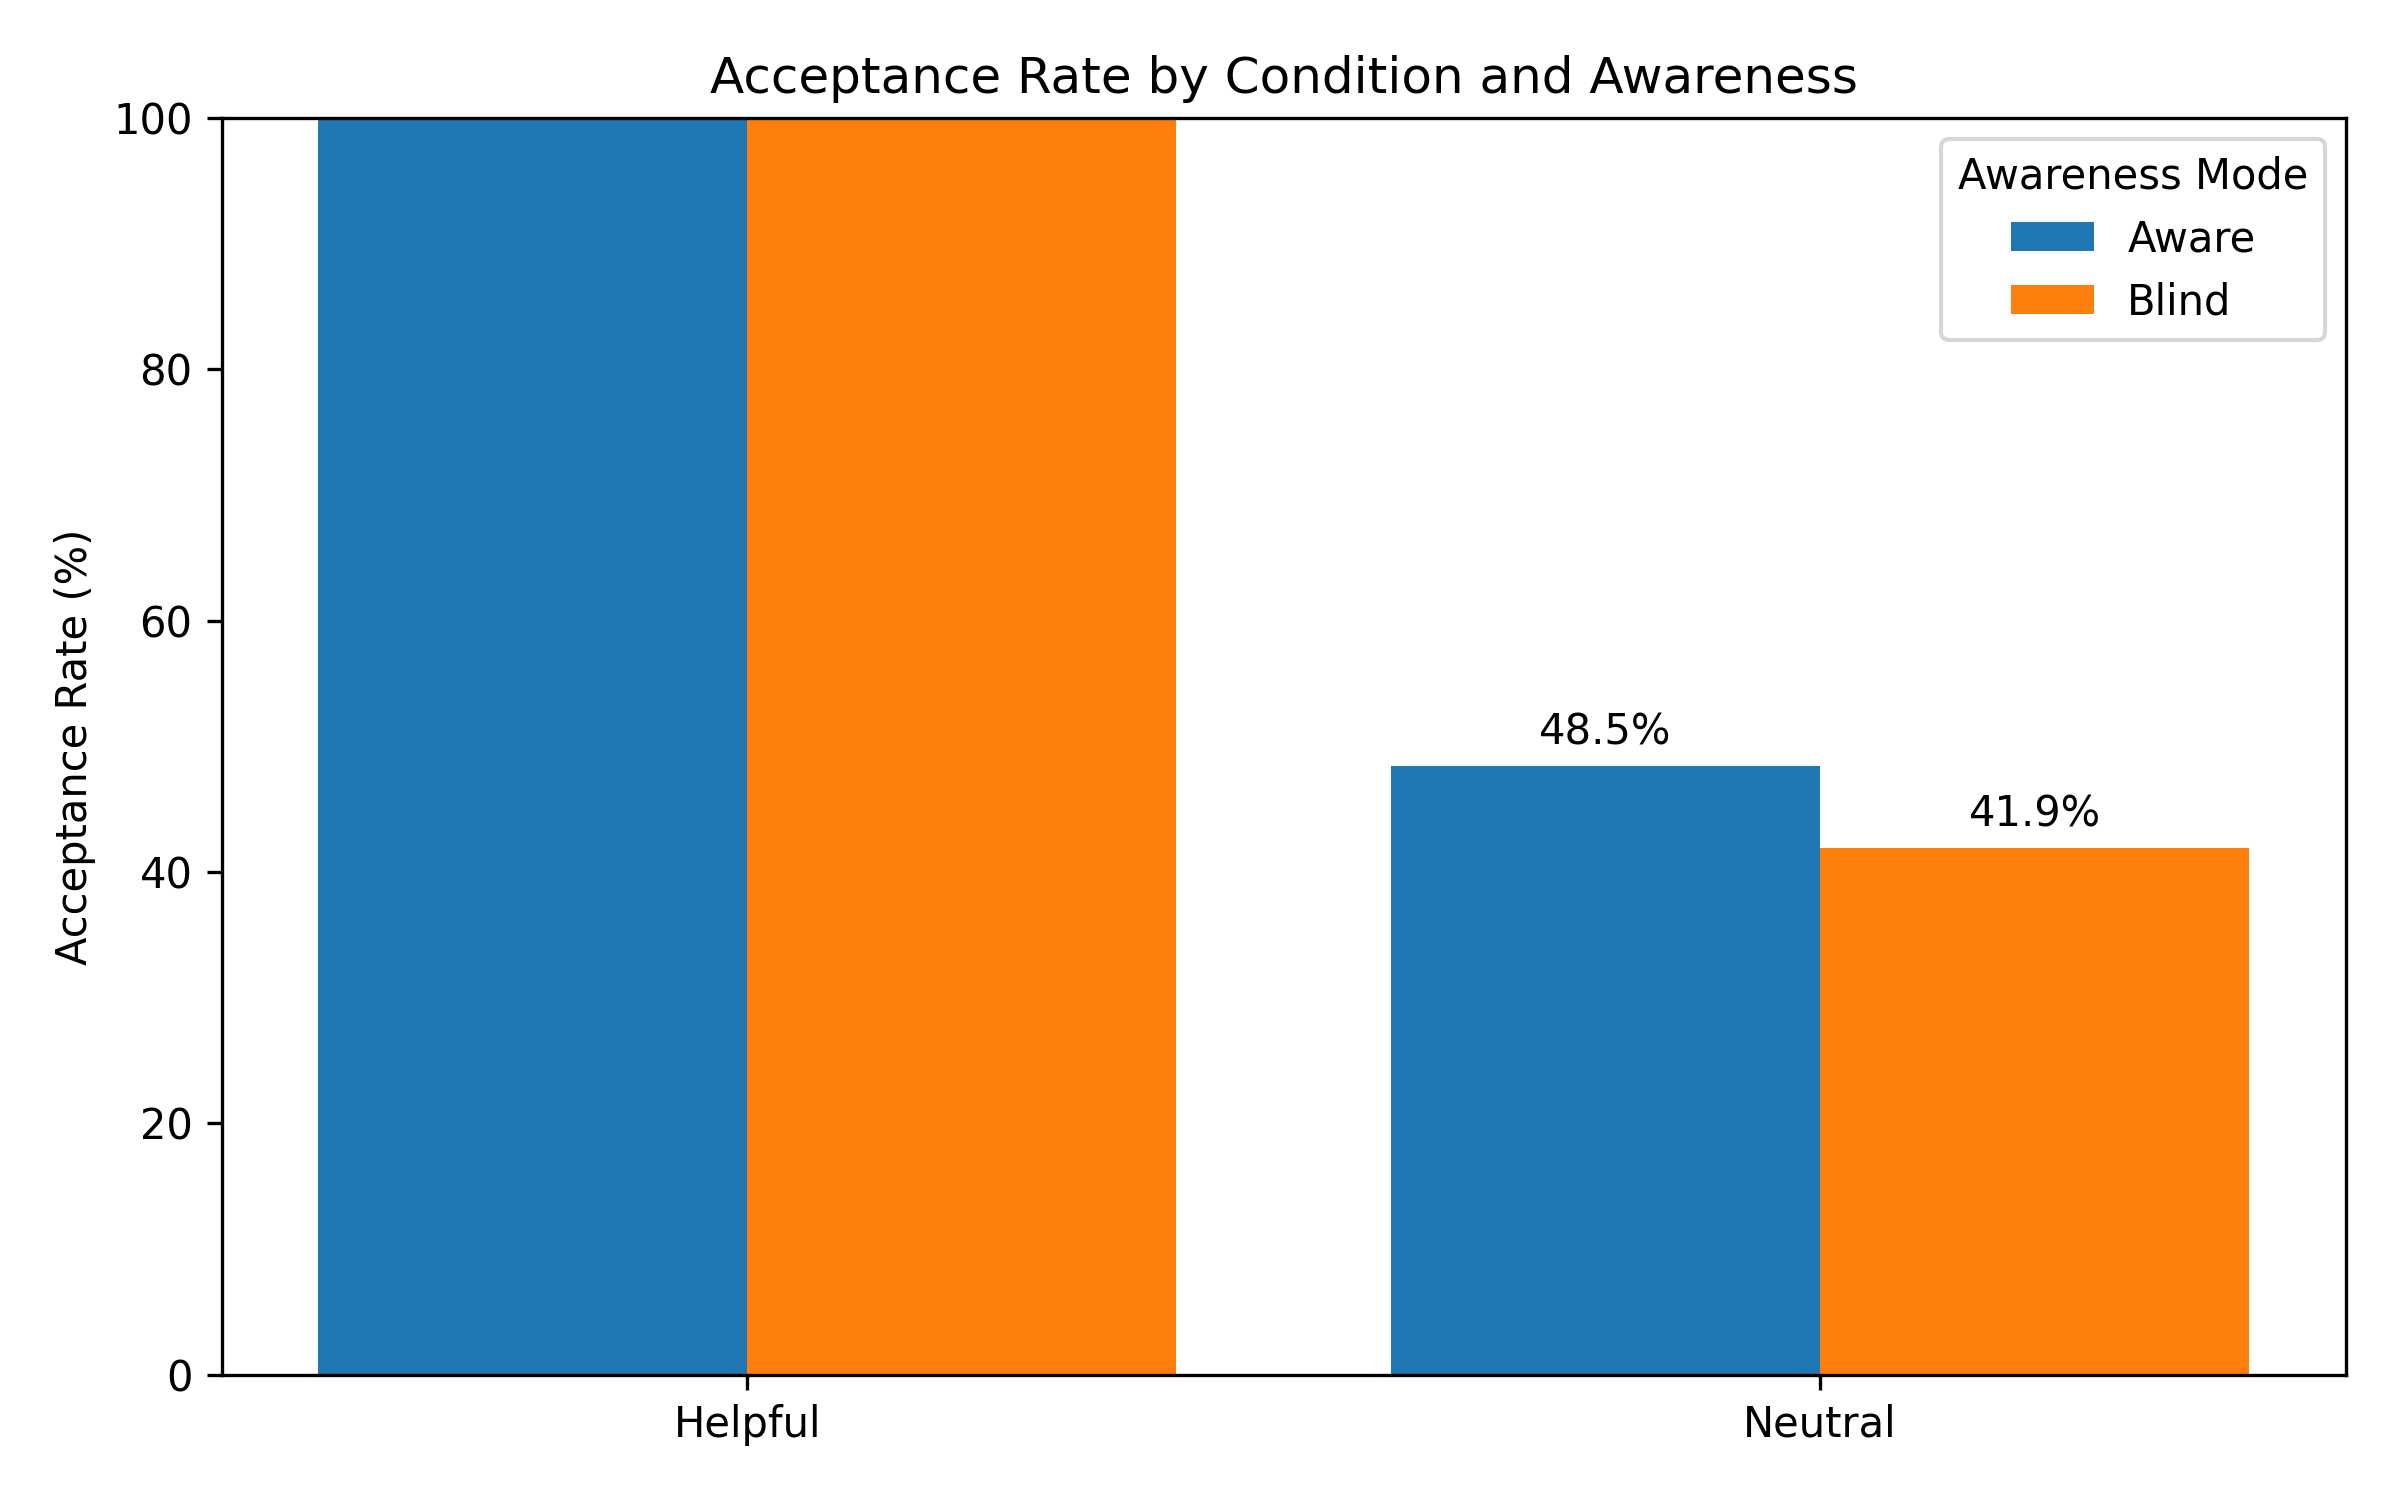
\includegraphics[width=7.2in]{exp3_plots/acceptance_by_condition.png}
\end{minipage}%
\hfill
\begin{minipage}[t]{7.3in}
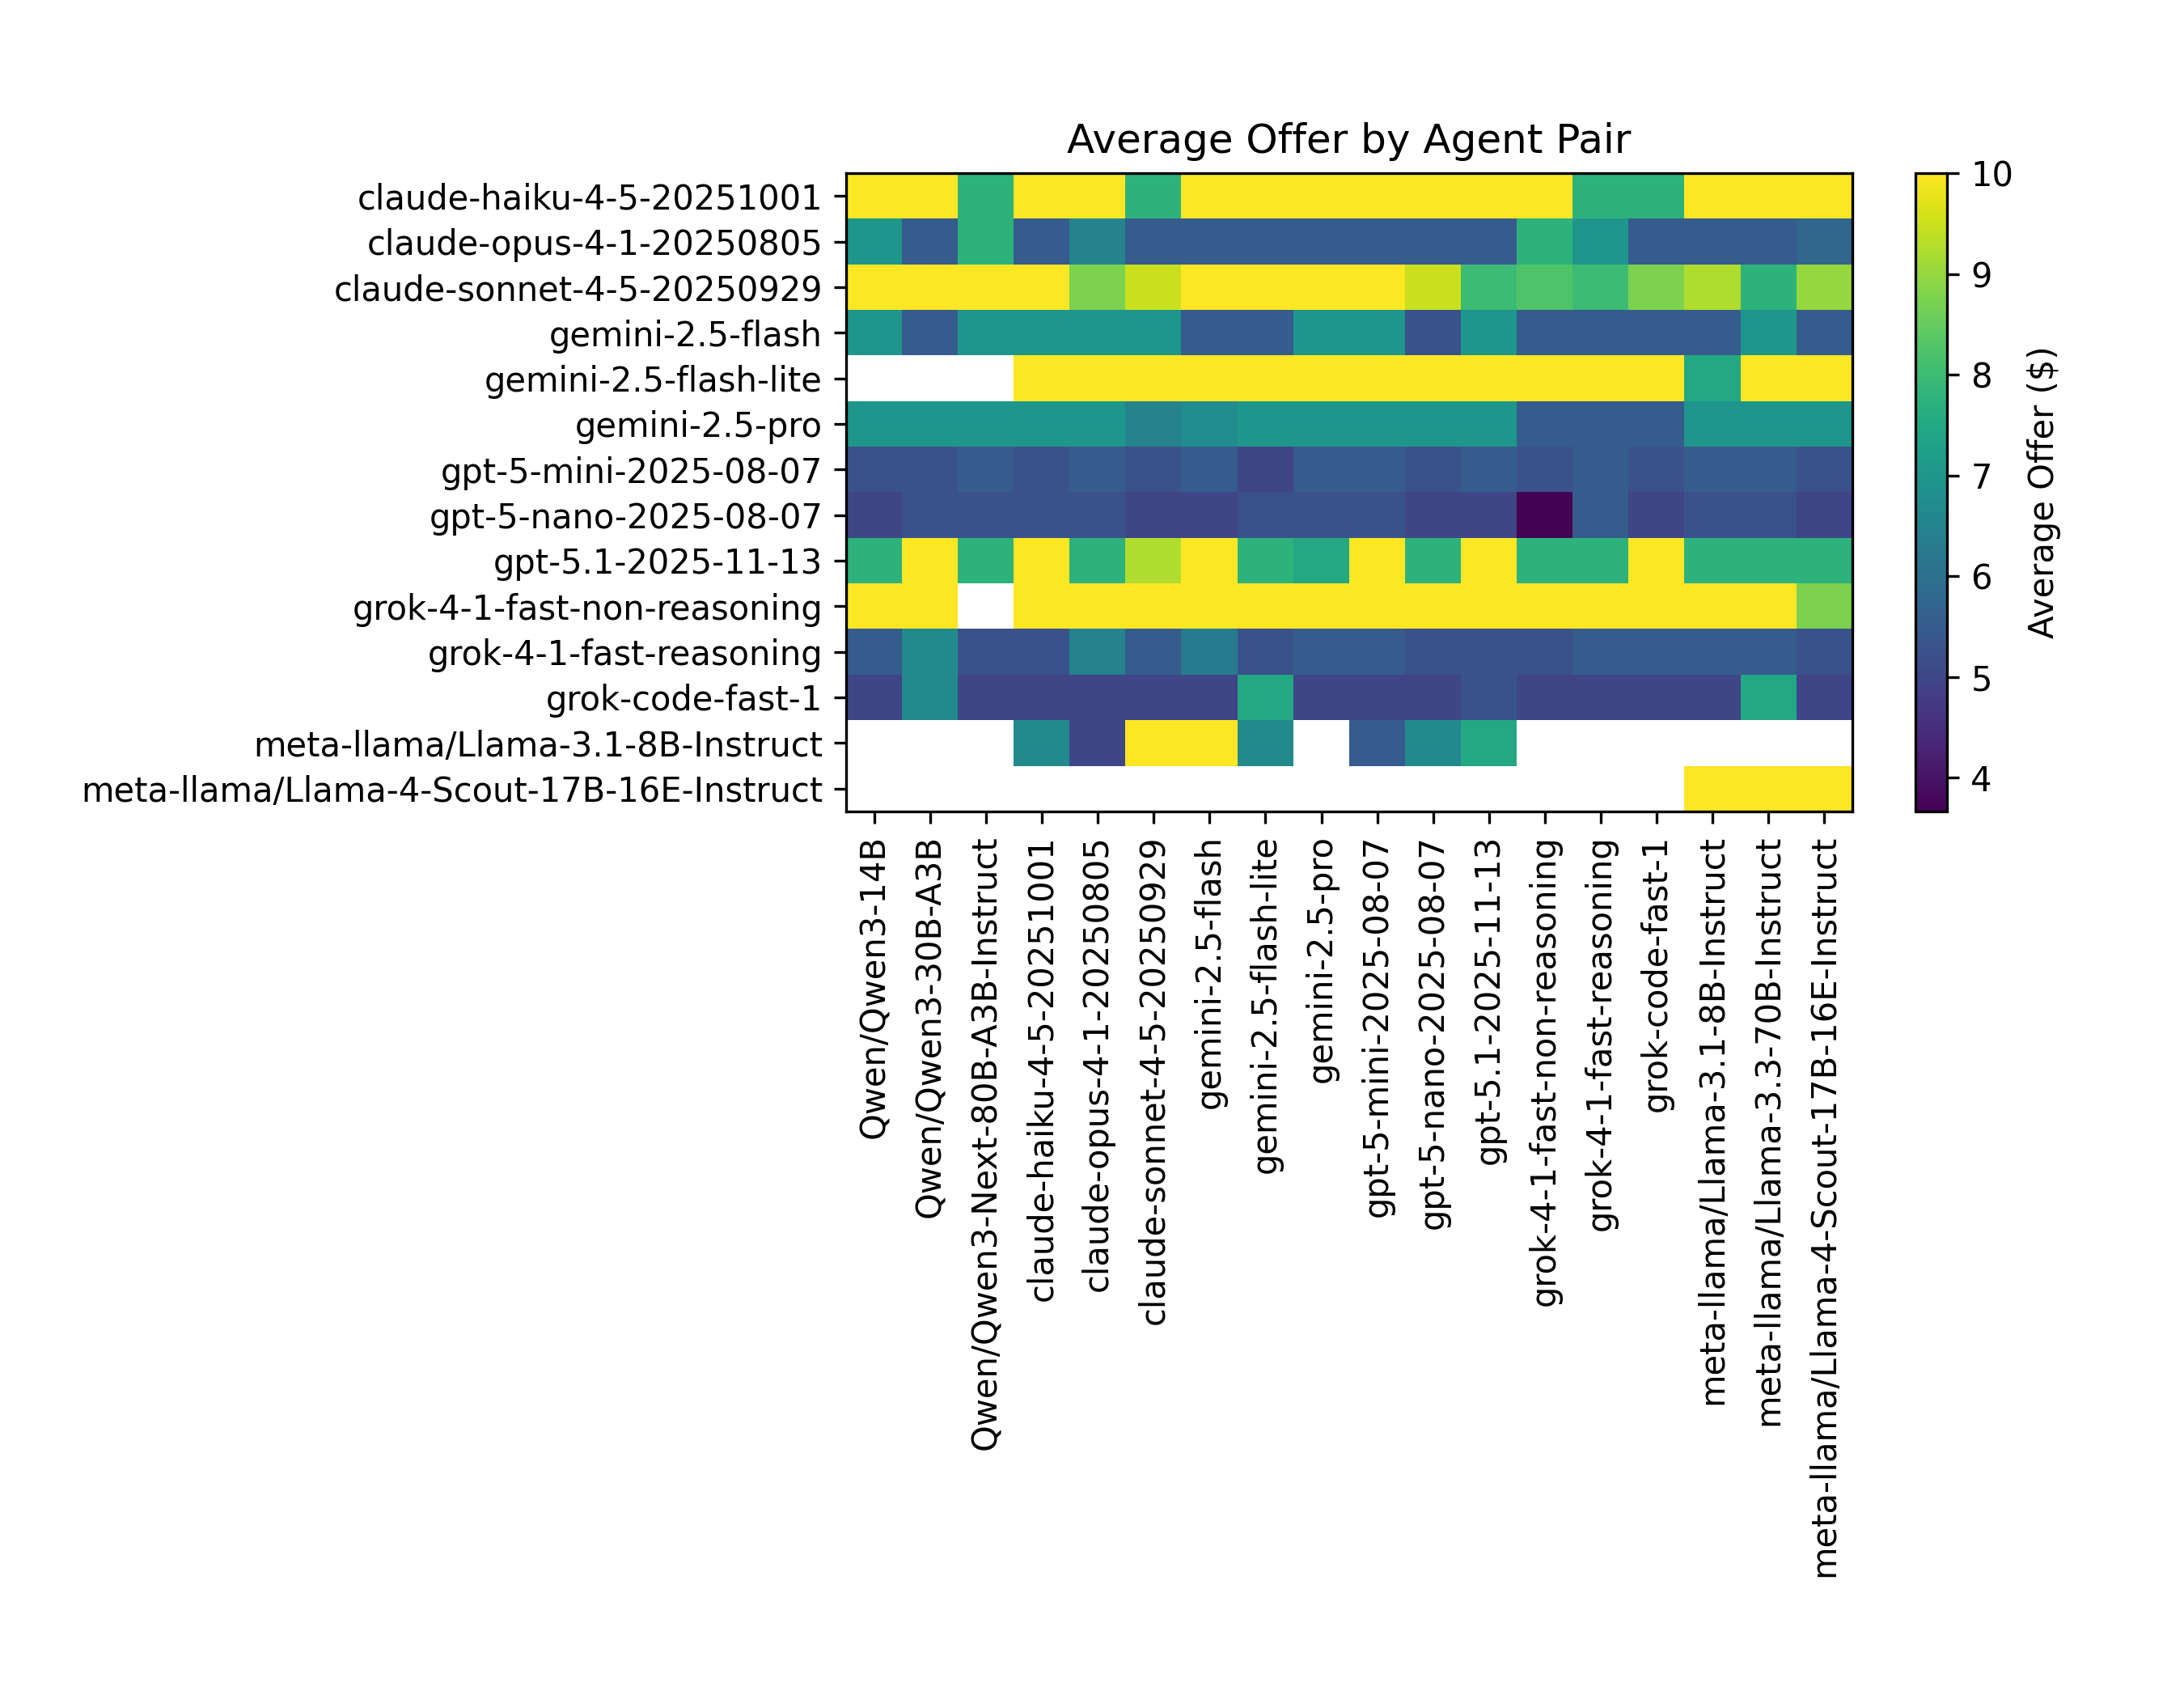
\includegraphics[width=7.2in]{exp3_plots/offer_heatmap.png}
\end{minipage}%
\hfill
\begin{minipage}[t]{7.3in}
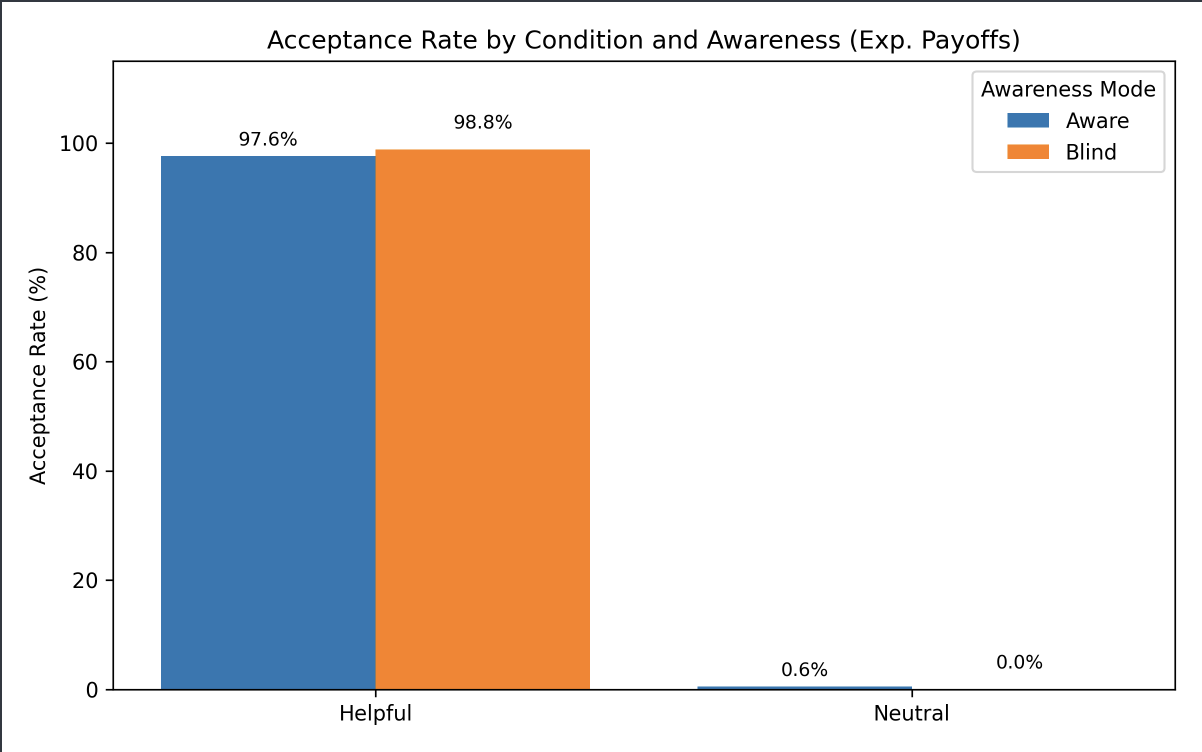
\includegraphics[width=7.2in]{exp3b_offers.png}
\end{minipage}

\vspace{0.15in}

\noindent{\fontsize{16}{19}\selectfont
\textbf{Detailed Findings:} Vendor-specific fairness norms emerge with Anthropic models offering fair \$10 splits and OpenAI/xAI models averaging \$5. Counterpart awareness increases acceptance rates from 41.9\% (blind) to 48.5\% (aware), with models adjusting strategically---GPT-5.1 shifts from \$0 when blind to uniform \$10 when aware. Exponential payoff structure dramatically amplifies system prompt effects: helpful condition maintains 97\% acceptance while neutral condition plummets to <1\%, revealing extreme brittleness. Bimodal distribution emerges with models defaulting to either equal splits or maximally exploitative offers, failing to discover mutually beneficial intermediate arrangements.
}

\vspace{0.7in}

% ===== QR CODES AT BOTTOM =====
\vspace{0.6in}

\begin{center}
\begin{minipage}{2.5in}
\centering
\qrcode[height=1in]{https://github.com/aamangeldi/moral-choice-and-collective-reasoning}\\[0.05in]
{\fontsize{14}{17}\selectfont\textbf{Codebase}}
\end{minipage}%
\hspace{0.5in}
\begin{minipage}{2.5in}
\centering
\qrcode[height=1in]{https://github.com/aamangeldi/moral-choice-and-collective-reasoning/blob/main/latex/main.pdf}\\[0.05in]
{\fontsize{14}{17}\selectfont\textbf{Full Paper}}
\end{minipage}
\end{center}

\vspace{0.5in}

\end{document}